The cart layer consists of the hardware components of the cart as well as the switches. The switches include a manual mode switch to remove autonomous activity and a killswitch to immediately unpower the cart.

\begin{figure}[h!]
	\centering
 	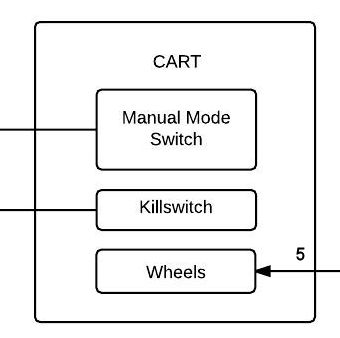
\includegraphics[width=0.60\textwidth]{images/cart}
 \caption{Cart layer}
\end{figure}

\subsection{Manual Mode Switch}
The manual mode switch subsystem will be used to ensure that the Smart Cart will not be autonomously moving.

\begin{figure}[h!]
	\centering
 	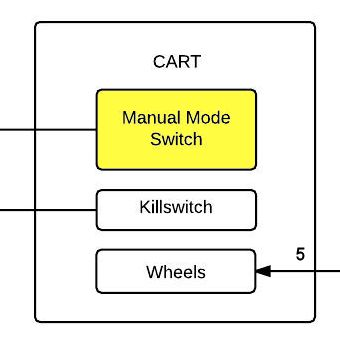
\includegraphics[width=0.60\textwidth]{images/cart_manual}
 \caption{Manual mode switch subsystem}
\end{figure}

\subsubsection{Assumptions}
Assumptions made are as follows:
\begin{itemize}
	\item The manual mode switch subsystem will ensure the safety of the users and people around the user.
	\item The manual mode switch subsystem will not power the Smart Cart off, but simply disable autnomous smovement.
\end{itemize}

\subsubsection{Responsibilities}
The manual mode switch subsystem's responsibilities are as follows:
\begin{itemize}
	\item The switch will disable the autonomous movement of the cart.
	\item The switch will ensure the safety of the user and surrounding people.
\end{itemize}

\subsubsection{Subsystem Interfaces}

\begin {table}[H]
\caption {Manual mode switch subsystem interfaces} 
\begin{center}
    \begin{tabular}{ | p{1cm} | p{6cm} | p{3cm} | p{3cm} |}
    \hline
    ID & Description & Inputs & Outputs \\ \hline
    \ N/A & Disable converter & \pbox{3cm}{N/A} & \pbox{3cm}{Voltage converter}  \\ \hline
    \end{tabular}
\end{center}
\end{table}
\newline


\subsection{Killswitch}
The killswitch subsystem will be used to ensure that the Smart Cart will be immediately turned off.

\begin{figure}[h!]
	\centering
 	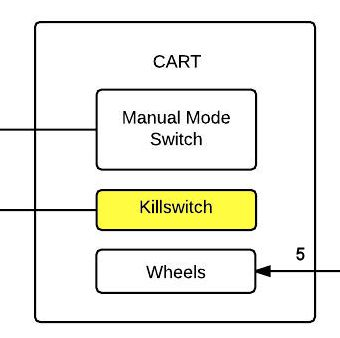
\includegraphics[width=0.60\textwidth]{images/cart_kill}
 \caption{Killswitch subsystem}
\end{figure}

\subsubsection{Assumptions}
Assumptions made are as follows:
\begin{itemize}
	\item Power to the Smart Cart components will be disabled.
	\item Power to external tools and equipment will be disabled.
\end{itemize}

\subsubsection{Responsibilities}
The killswitch subsystem's responsibilities are as follows:
\begin{itemize}
	\item The switch will disable the battery from powering the Smart Cart and its components.
\end{itemize}

\subsubsection{Subsystem Interfaces}

\begin {table}[H]
\caption {Killswitch subsystem interfaces} 
\begin{center}
    \begin{tabular}{ | p{1cm} | p{6cm} | p{3cm} | p{3cm} |}
    \hline
    ID & Description & Inputs & Outputs \\ \hline
    \ N/A & Disable battery & \pbox{3cm}{N/A} & \pbox{3cm}{Deep cycle battery}  \\ \hline
    \end{tabular}
\end{center}
\end{table}
\newline


\subsection{Wheels}
The wheels subsystem will be used to provide movement to the Smart Cart. The wheels will be controlled by the Crab Drive layer.

\begin{figure}[h!]
	\centering
 	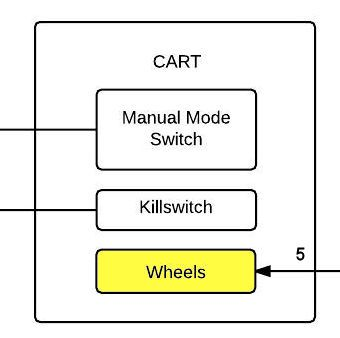
\includegraphics[width=0.60\textwidth]{images/cart_wheel}
 \caption{Wheels subsystem}
\end{figure}

\subsubsection{Assumptions}
Assumptions made are as follows:
\begin{itemize}
	\item The wheels must be able to turn in any sort of direction.
	\item The wheels will move together as a whole.
\end{itemize}

\subsubsection{Responsibilities}
The wheels subsystem's responsibilities are as follows:
\begin{itemize}
	\item The wheels will be able to withstand movement through rough terrain.
	\item The wheels' movement and direction will be controlled by the wheel motors.
\end{itemize}

\subsubsection{Subsystem Interfaces}

\begin {table}[H]
\caption {Wheel subsystem interfaces} 
\begin{center}
    \begin{tabular}{ | p{1cm} | p{6cm} | p{3cm} | p{3cm} |}
    \hline
    ID & Description & Inputs & Outputs \\ \hline
    \#5 & Move wheels & \pbox{3cm}{Wheel motors} & \pbox{3cm}{N/A}  \\ \hline
    \end{tabular}
\end{center}
\end{table}
